%% (C) 2021 Pablo Alvarado
%% Escuela de Ingeniería Electrónica
%% Plantila para presentaciones

%\documentclass[15pt,compressed]{beamer} % [12pt]
\documentclass[10pt,aspectratio=169]{beamer} % [12pt]
\usepackage{colortbl}
\usepackage{graphicx}
\usepackage{multirow}
%\usepackage{fontspec}
\usepackage[spanish]{babel}
\usepackage[utf8]{inputenc}
\usepackage[scaled]{helvet}
\renewcommand\familydefault{\sfdefault} 
\usepackage[T1]{fontenc}
\usepackage{textcomp}
\usepackage{multicol}
\usepackage{array}                      % extensions to tabular environment
\usepackage{tabularx}                   % supports tables with fixed width
\usepackage{booktabs}
\usepackage{rotating}
\usepackage{trsym} %% Para simbolos de transformadas o---o
\usepackage{ifthen}
\usepackage{listings}
\usepackage{algorithm2e}
\usepackage{algorithmic}
\usepackage{icomma}
\usepackage{mathtools}
\usepackage{amsmath}
\usepackage{amssymb}
\usepackage{amstext}
\usepackage{bm}   %% Bold math

% Configuration of listings
\lstset{%
  basicstyle=\scriptsize,
  commentstyle=\color{blue}
}
\lstset{literate=%
  {á}{{\'a}}1
  {é}{{\'e}}1
  {í}{{\'i}}1
  {ó}{{\'o}}1
  {ú}{{\'u}}1
  {ñ}{{\~n}}1
  {Á}{{\'A}}1
  {É}{{\'E}}1
  {Í}{{\'I}}1
  {Ó}{{\'O}}1
  {Ú}{{\'U}}1
  {Ñ}{{\~N}}1
}

\definecolor{links}{HTML}{2A1B81}
\hypersetup{colorlinks,linkcolor=,urlcolor=links}

\DeclareMathAlphabet{\mathpzc}{OT1}{pzc}{m}{it}
\DeclareMathAlphabet{\mathpss}{OT1}{cmss}{m}{sl}

\usetheme[width=25mm]{Marburg}   % Barra azul a la derecha
\usecolortheme{tec}

\addtobeamertemplate{navigation symbols}{}{%
    \usebeamerfont{footline}%
    \usebeamercolor[fg]{footline}%
    \hspace{1em}%
    \raisebox{1pt}{\insertframenumber/\inserttotalframenumber}
}

\definecolor{tecAzul}{RGB}{31,47,95}      % según manual de imagen 2016
\definecolor{tecRojo}{RGB}{239,64,52}     % según manual de imagen 2016
\definecolor{tecNaranja}{RGB}{255,174,57} % según manual de imagen 2016
\definecolor{tecVerde}{RGB}{133,189,64}   % según manual de imagen 2016
\definecolor{tecCian}{RGB}{37,158,205}    % según manual de imagen 2016
\definecolor{tecTurq}{RGB}{35,168,156}    % según manual de imagen 2016

\definecolor{dkred}{RGB}{239,64,52}       % dark red
\definecolor{dkgreen}{RGB}{133,189,64}    % dark green
\definecolor{dkblue}{RGB}{31,47,95}       % dark blue
\definecolor{dkgray}{gray}{0.4}           % dark gray
\definecolor{ltgray}{gray}{0.75}          % light gray
\definecolor{dkmagenta}{rgb}{0.3,0.0,0.3} % dark magenta
\definecolor{ltyellow}{RGB}{251,75,58}    % light yellow
\definecolor{dkyellow}{RGB}{255,174,57}   % dark yellow
\definecolor{dkcyan}{RGB}{37,158,205}     % dark cyan
\definecolor{ltcyan}{rgb}{0.7,1,1}        % light cyan

\newcommand*{\vcenteredhbox}[1]{\begingroup
\setbox0=\hbox{#1}\parbox{\wd0}{\box0}\endgroup}

\newcommand{\bG}[1]{\textcolor{dkgreen}{\textbf{#1}}}
\newcommand{\bR}[1]{\textcolor{dkred}{\textbf{#1}}}
\newcommand{\bB}[1]{\textcolor{dkblue}{\textbf{#1}}}
\newcommand{\bM}[1]{\textcolor{dkmagenta}{\textbf{#1}}}
\newcommand{\bY}[1]{\textcolor{dkyellow}{\textbf{#1}}}
\newcommand{\bC}[1]{\textcolor{dkcyan}{\textbf{#1}}}

\newcommand{\iG}[1]{\textcolor{dkgreen}{\emph{#1}}}
\newcommand{\iR}[1]{\textcolor{dkred}{\emph{#1}}}
\newcommand{\iB}[1]{\textcolor{dkblue}{\emph{#1}}}
\newcommand{\iM}[1]{\textcolor{dkmagenta}{\emph{#1}}}
\newcommand{\iY}[1]{\textcolor{dkyellow}{\emph{#1}}}
\newcommand{\iC}[1]{\textcolor{dkcyan}{\emph{#1}}}

\newcommand{\nG}[1]{\textcolor{dkgreen}{{#1}}}
\newcommand{\nlG}[1]{\textcolor{ltgray}{{#1}}}
\newcommand{\ndG}[1]{\textcolor{dkgray}{{#1}}}
\newcommand{\nR}[1]{\textcolor{dkred}{{#1}}}
\newcommand{\nB}[1]{\textcolor{dkblue}{{#1}}}
\newcommand{\nM}[1]{\textcolor{dkmagenta}{{#1}}}
\newcommand{\nY}[1]{\textcolor{dkyellow}{{#1}}}
\newcommand{\nC}[1]{\textcolor{dkcyan}{{#1}}}


%%%%%%%%%%%%%%%%%%%%%%%%%%%%%%%%%%%%%%%%%%%%%%%%%%%%%%%%%%%%%%%%%%%%%%%%%%%%
%  Notación

\usepackage{mathrsfs}                   % Calygraphic fonts for transforms

%%%%%%%%%%%%%%%%%%%%%%%%%%%%%%%%%%%%%%%%%%%%%%%%%%%%%%%%%%%%%%%%%%%%%%%%%%%%

\def\hilite<#1>{%
  \temporal<#1>{\color{tecAzul!20!white}}{\color{tecRojo}}{\color{black}}}

\newcommand{\centrar}[1]{%
\begin{center}
  #1
\end{center}%
}

\deftranslation[to=spanish]{Example}{Ejemplo}
\deftranslation[to=spanish]{Definition}{Definición}

\newenvironment{exampleframe}[1][nothing]{
  \begin{frame}[allowframebreaks]
    \ifthenelse{\equal{#1}{nothing}}{
      \frametitle{Ejemplo}
    }{
      \frametitle{Ejemplo: #1}
    }
}{
  \end{frame}
}

\newcommand{\cleft}[2][.]{%
  \begingroup\colorlet{savedleftcolor}{.}%
  \color{#1}\left#2\color{savedleftcolor}%
}
\newcommand{\cright}[2][.]{%
  \color{#1}\right#2\endgroup
}


% What is this all about:
\title[Proyecto Final de Graduación]{Desarrollo de un conjunto de flujos de trabajo \\
                                  para la implementación de software embebido \\ 
                                  a bordo de computadoras de guía, navegación \\
                                  y control espacial}
\institute[TEC]{Escuela de Ingeniería Electrónica \\ Tecnológico de Costa Rica}
\date[Noviembre 2023]{15 de noviembre, 2024}
%% Si ya usted tiene un título previo, úselo (p.\,ej. Ing.\,Juan Pérez Pérez)
\author[D.\ Duarte]{David Duarte}

%  Notación

%% (C) 2021 Pablo Alvarado
%% Escuela de Ingeniería Electrónica
%% Plantila para presentaciones
%% notation.tex
%% ---------------------------------------------------------------------------

%%
% Command definitions for localized symbol format definition
%%
\renewcommand{\Re}{\operatorname{Re}}
\renewcommand{\Im}{\operatorname{Im}}
\newcommand{\notimplies}{%
  \mathrel{{\ooalign{\hidewidth$\not\phantom{=}$\hidewidth\cr$\implies$}}}}

\newcommand{\prt}[1]{\ensuremath{\mathcal{#1}}}         %% partitioning
\newcommand{\img}[1]{\ensuremath{\mathcal{#1}}}         %% image as a set
\newcommand{\reg}[1][R]{\ensuremath{\mathcal{#1}}}      %% region
\newcommand{\pred}[1]{\ensuremath{\mathrm{#1}}}         %% predicate
\newcommand{\operat}[2]{\mathcal{#1}\left\{#2\right\}}
\newcommand{\transf}[1]{\mathscr{#1}}
\newcommand{\fourier}[1]{\transf{F}\left\{#1\right\}}
\newcommand{\ifourier}[1]{\transf{F}^{-1}\left\{#1\right\}}
\newcommand{\laplace}[1]{\transf{L}\left\{#1\right\}}
\newcommand{\ulaplace}[1]{\transf{L}_u\left\{#1\right\}}
\newcommand{\blaplace}[1]{\transf{L}_b\left\{#1\right\}}
\newcommand{\ilaplace}[1]{\transf{L}^{-1}\left\{#1\right\}}
\newcommand{\ztrans}[1]{\transf{Z}\left\{#1\right\}}
\newcommand{\iztrans}[1]{\transf{Z}^{-1}\left\{#1\right\}}
\newcommand{\zutrans}[1]{\transf{Z}_u\left\{#1\right\}}
\newcommand{\exceq}{\ensuremath{\overset{!}{=}}}

\newcommand{\tr}[1]{\operatorname{tr}\!\left\{#1\right\}}
\newcommand{\rank}{\operatorname{rg}}
\newcommand{\trace}[1]{\operatorname{tr}{#1}}
\newcommand{\signum}{\operatorname{signum}}
\newcommand{\pos}{\operatorname{pos}}
\newcommand{\val}{\operatorname{val}}
\newcommand{\Var}{\operatorname{Var}}
\newcommand{\Cov}{\operatorname{Cov}}
\newcommand{\Curt}{\operatorname{Curt}} % Curtosis
\newcommand{\E}{\operatorname{E}}
\newcommand{\ind}[1]{1\!\left\{#1\right\}} % indicator function
\newcommand{\vct}[1]{\ensuremath{\underline{\bm{{#1}}}}}
\newcommand{\pix}[1]{\ensuremath{\bm{#1}}}
\newcommand{\mat}[1]{\ensuremath{\bm{{#1}}}}
\newcommand{\tsr}[1]{\ensuremath{\mathcal{#1}}}
\newcommand{\jacob}{\ensuremath{\bm{J}}} % Jacobian
\newcommand{\VC}{\operatorname{VC}} % Vapnik-Chervonenkis
\newcommand{\MI}{\operatorname{MI}} % Mutual information
\newcommand{\KL}{\operatorname{KL}} % Kullback-Leibler
\newcommand{\MAP}{\operatorname{MAP}} % Maximum a posteriori

\newcommand{\vctOmega}{\vct{\bm{\Omega}}}
\newcommand{\vctalpha}{\vct{\bm{\alpha}}}
\newcommand{\vctbeta}{\vct{\bm{\beta}}}
\newcommand{\vctgamma}{\vct{\bm{\gamma}}}
\newcommand{\vcteta}{\vct{\bm{\eta}}}
\newcommand{\vctmu}{\vct{\bm{\mu}}}
\newcommand{\vctomega}{\vct{\bm{\omega}}}
\newcommand{\vctphi}{\vct{\bm{\phi}}}
\newcommand{\vctpsi}{\vct{\bm{\psi}}}
\newcommand{\vctpi}{\vct{\bm{\pi}}}
\newcommand{\vcttheta}{\vct{\bm{\theta}}}
\newcommand{\vctvarphi}{\vct{\bm{\varphi}}}
\newcommand{\vctsigma}{\vct{\bm{\sigma}}}
\newcommand{\vctxi}{\vct{\bm{\xi}}}
\newcommand{\vctzeta}{\vct{\bm{\zeta}}}
\newcommand{\vctvarepsilon}{\vct{\bm{\varepsilon}}}

\newcommand{\raum}[1]{\ensuremath{\mathbb{#1}}}

\newcommand{\matGamma}{\mat{\bm{\Gamma}}}
\newcommand{\matLambda}{\mat{\bm{\Lambda}}}
\newcommand{\matPhi}{\mat{\bm{\Phi}}}
\newcommand{\matPi}{\mat{\bm{\Pi}}}
\newcommand{\matPsi}{\mat{\bm{\Psi}}}
\newcommand{\matSigma}{\mat{\bm{\Sigma}}}
\newcommand{\matTheta}{\mat{\bm{\Theta}}}

\newcommand{\row}[2]{\ensuremath{\underline{\bm{#1}}_{#2,:}}}
\newcommand{\col}[2]{\ensuremath{\underline{\bm{#1}}_{:,#2}}}
\newcommand{\seq}[1]{\ensuremath{#1}}
\newcommand{\set}[1]{\ensuremath{\mathcal{#1}}}
\newcommand{\gset}[1]{\ensuremath{#1}} %% set for greek symbols
\newcommand{\front}[1]{\widehat{\set{#1}}}
\newcommand{\setlambda}{\set{\bm{\lambda}}}
\newcommand{\klass}[1]{\ensuremath{\mathpss{#1}}}
\newcommand{\graph}[1]{\ensuremath{\mathsf{#1}}}
\newcommand{\lab}[1]{\ensuremath{\mathpss{L}(#1)}}
\newcommand{\myfrac}[2]{{\footnotesize #1/#2}}
\newcommand{\ifthenspc}{\rule{3mm}{0mm}}
\newcommand{\point}[1]{\ensuremath{\mathsf{#1}}}
\newcommand{\estim}[1]{\ensuremath{\hat{#1}}}
\newcommand{\numset}[1]{\ensuremath{\mathbb{#1}}}
\newcommand{\tuple}[1]{\ensuremath{\left\langle#1\right\rangle}}
\newcommand{\conj}[1]{\ensuremath{{{#1}^{\ast}}}}
\newcommand{\base}[1]{\set{#1}}
\newcommand{\zeron}[1]{\ensuremath{\underset{\uparrow}{#1}}}
\newcommand{\sysT}{\ensuremath{\mathcal{T}}}
\newcommand{\sys}[1]{\ensuremath{\sysT\left\{#1\right\}}}
%\newcommand{\sen}{\operatorname{sen}} % sinus in spanish (seno)
%\newcommand{\senh}{\operatorname{senh}} % sinus hiperbolicus in spanish (seno)
%\newcommand{\arcsen}{\operatorname{arcsen}} % arcus sinus hiperbolicus in spanish (arcoseno)
\newcommand{\sgn}{\operatorname{sgn}} % signus
\newcommand{\roc}{\text{ROC: }}
\newcommand{\med}{\operatorname{med}} % median
\newcommand{\diag}{\operatorname{diag}} % diagonal
\newcommand{\normal}{\ensuremath{\mathcal{N}}}
\newcommand{\binomial}{\ensuremath{\mathcal{B}}}
\newcommand{\multinomial}{\ensuremath{\operatorname{Multinomial}}}
\newcommand{\Bernoulli}{\operatorname{Ber}}
\newcommand{\drawn}{\thicksim}

\newcommand{\lagr}{\ensuremath{\mathcal{L}}}
\newcommand{\primal}{\ensuremath{\mathcal{P}}}
\newcommand{\original}{\ensuremath{\mathcal{P}}}
\newcommand{\dual}{\ensuremath{\mathcal{D}}}

\newcommand{\code}[1]{\texttt{#1}}
\newcommand{\conv}{\ensuremath{\ast}}
\newcommand{\corr}{\ensuremath{\circ}}
\newcommand{\cconv}{\ensuremath{\;\,\text{\footnotesize{N}}\!\!\!\!\!\!\bigcirc}}
\newcommand{\Ln}{\operatorname{Ln}}
\newcommand{\sa}{\operatorname{sa}}
\newcommand{\senc}{\operatorname{senc}}
\newcommand{\si}{\operatorname{si}}


%% Natural, Integer and Real Numbers
\newcommand{\setA}{\ensuremath{\mathbb{A}}}
\newcommand{\setB}{\ensuremath{\mathrm{I\negthinspace B}}}
\newcommand{\setC}{\ensuremath{\mathbb{C}}}
\newcommand{\setD}{\ensuremath{\mathrm{I\negthinspace D}}}
\newcommand{\setE}{\ensuremath{\mathrm{I\negthinspace E}}}
\newcommand{\setF}{\ensuremath{\mathrm{I\negthinspace F}}}
\newcommand{\setG}{\ensuremath{\mathbb{G}}}
\newcommand{\setH}{\ensuremath{\mathrm{I\negthinspace H}}}
\newcommand{\setI}{\ensuremath{\mathbb{I}}}
\newcommand{\setJ}{\ensuremath{\mathbb{J}}}
\newcommand{\setK}{\ensuremath{\mathrm{I\negthinspace K}}}
\newcommand{\setL}{\ensuremath{\mathrm{I\negthinspace L}}}
\newcommand{\setM}{\ensuremath{\mathrm{I\negthinspace M}}}
\newcommand{\setN}{\ensuremath{\mathrm{I\negthinspace N}}}
\newcommand{\setO}{\ensuremath{\mathbb{O}}}
\newcommand{\setP}{\ensuremath{\mathrm{I\negthinspace P}}}
\newcommand{\setQ}{\ensuremath{\mathbb{Q}}}
\newcommand{\setR}{\ensuremath{\mathrm{I\negthinspace R}}}
\newcommand{\setS}{\ensuremath{\mathbb{S}}}
\newcommand{\setT}{\ensuremath{\mathbb{T}}}
\newcommand{\setU}{\ensuremath{\mathbb{U}}}
\newcommand{\setV}{\ensuremath{\mathbb{V}}}
\newcommand{\setW}{\ensuremath{\mathbb{W}}}
\newcommand{\setX}{\ensuremath{\mathbb{X}}}
\newcommand{\setY}{\ensuremath{\mathbb{Y}}}
\newcommand{\setZ}{\ensuremath{\mathbb{Z}}}

\newcommand{\orden}{\ensuremath{\mathcal{O}}}
\newcommand{\order}{\ensuremath{\mathcal{O}}}
\newcommand{\loss}{\ensuremath{\mathcal{L}}}

%%
% Multimap symbols
%
\newcommand{\ttoF}{\TransformHoriz}
\newcommand{\Ftot}{\InversTransformHoriz}
\newcommand{\ttoZ}{\ttoF}
\newcommand{\Ztot}{\Ftot}
\newcommand{\ttoZu}{\overset{z_u}{\ttoF}}
\newcommand{\Zutot}{\overset{z_u}{\Ftot}}
\newcommand{\vttoF}{\text{\begin{sideways}$\Ftot$\end{sideways}}}
\newcommand{\vFtot}{\text{\begin{sideways}$\ttoF$\end{sideways}}}
\newcommand{\vttoZ}{\vttoF}
\newcommand{\vZtot}{\vFtot}
\newcommand{\ttoDF}{\underset{N}{\ttoF}}
\newcommand{\DFtot}{\underset{N}{\Ftot}}

\newcommand{\thisis}[2]{\underset{#1}{\underbrace{#2}}}

\newcommand\givenbase[1][]{\:#1\lvert\:}
\let\given\givenbase
\newcommand\sgiven{\givenbase[\delimsize]}
\DeclarePairedDelimiterX\Basics[1](){\let\given\sgiven #1}


%%%%%%%%%%%%%%%%%%%%%%%%%%%%%%%%%%%%%%%%%%%%%%%%%%%%%%%%%%%%%%%%%%%%%%%%%%%%

\begin{document}
\graphicspath{{./}{./fig/}}

\begin{frame}
  \titlepage
\end{frame}


\begin{frame}{Agenda}
  \tableofcontents
\end{frame}

% Título para el contexto
\section{Contexto del proyecto}

\begin{frame}{Contexto del proyecto}
    \centering
    \includegraphics[scale=0.2]{logos/tec.png} \hfill
    \includegraphics[scale=0.3]{logos/seteclab.png} \hfill
    \parbox[c][3cm][c]{0.3\textwidth}{\centering ELaNAV \\ 2025}
\end{frame}

\section{Problema}

\begin{frame}{Contexto del problema}
  \centering
  \includegraphics[scale=0.3]{planteamineto_problema/problema.pdf}
\end{frame}

\subsection{Síntesis del problema}
\begin{frame}{Síntesis del problema}
  \begin{itemize}
    \item El SETEC-Lab no cuenta con un marco de trabajo que permita la implementación de algoritmos de navegación y control en plataformas de hardware embebido que sea configurable y que cuente con mecanismos de medición de su desempeño.
  \end{itemize}
\end{frame}

\section{Objetivo general}
\begin{frame}{Objetivo general}
  \begin{itemize}
  \item Desarrollar un conjunto de flujos de trabajo para la implementación de software 
  a bordo de computadoras de guía, navegación y control espacial.
  \end{itemize}
\end{frame}

\section{Objetivos específicos}
\begin{frame}{Objetivos específicos}
  \begin{enumerate}
    \item Identificar una plataforma de hardware para el desarrollo de un modelo de ingeniería de una computadora de navegación espacial.
    \item Establecer flujos de trabajo para el prototipado de algoritmos de control de orientación y navegación para aplicaciones espaciales 
          con hardware en el Lazo (HIL).
    \item Evaluar casos de uso de una computadora de navegación y control espacial mediante la implementación de una aplicación de 
          referencia demostrativa.
  \end{enumerate}
\end{frame}

\section{Solución}

\subsection{Enfoque metodológico}

\begin{frame}{Enfoque metodológico}
  \begin{itemize}
    \item Selección de plataforma de desarrollo para GNC.
    \item Diseño de los flujos de trabajo.
    \item Evaluación de los flujos de trabajo con casos de estudio orientados a los sistemas GNC.
  \end{itemize}
\end{frame}


\subsection{Selección de plataforma de desarrollo}

\begin{frame}{Selección de plataforma de desarrollo}
  \centering
  \includegraphics[scale=0.6]{Diagrama_general_del_proyecto/seleccion_tarjeta_desarrollo.pdf}
\end{frame}

\begin{frame}{Selección de plataforma de desarrollo}
  \centering
  Matriz de Pugh para seleccionar la tarjeta de desarrollo que mejor se adapte a los requerimientos del proyecto
  \begin{table}[h!]
    \centering
    \resizebox{\columnwidth}{!}{%
    \begin{tabular}{lccccc}
    \hline
    \multicolumn{1}{|l|}{Criterios} & \multicolumn{1}{l|}{Peso} & \multicolumn{1}{l|}{ZCU102} & \multicolumn{1}{l|}{AGX Xavier} & \multicolumn{1}{l|}{TMS320C6678} & \multicolumn{1}{l|}{ZedBoard} \\ \hline
    \multicolumn{1}{|l|}{Capacidad de   procesamiento} & \multicolumn{1}{c|}{15} & \multicolumn{1}{c|}{15} & \multicolumn{1}{c|}{15} & \multicolumn{1}{c|}{8} & \multicolumn{1}{c|}{10} \\ \hline
    \multicolumn{1}{|l|}{Soporte para   sensores} & \multicolumn{1}{c|}{15} & \multicolumn{1}{c|}{15} & \multicolumn{1}{c|}{15} & \multicolumn{1}{c|}{15} & \multicolumn{1}{c|}{15} \\ \hline
    \multicolumn{1}{|l|}{Soporte para   actuadores} & \multicolumn{1}{c|}{10} & \multicolumn{1}{c|}{10} & \multicolumn{1}{c|}{10} & \multicolumn{1}{c|}{10} & \multicolumn{1}{c|}{10} \\ \hline
    \multicolumn{1}{|l|}{Soporte de   sistemas de tiempo real} & \multicolumn{1}{c|}{20} & \multicolumn{1}{c|}{20} & \multicolumn{1}{c|}{20} & \multicolumn{1}{c|}{15} & \multicolumn{1}{c|}{20} \\ \hline
    \multicolumn{1}{|l|}{Características   Físicas} & \multicolumn{1}{c|}{10} & \multicolumn{1}{c|}{4} & \multicolumn{1}{c|}{7} & \multicolumn{1}{c|}{10} & \multicolumn{1}{c|}{10} \\ \hline
    \multicolumn{1}{|l|}{Costo de la   tarjeta} & \multicolumn{1}{c|}{10} & \multicolumn{1}{c|}{7} & \multicolumn{1}{c|}{7} & \multicolumn{1}{c|}{7} & \multicolumn{1}{c|}{10} \\ \hline
    \multicolumn{1}{|l|}{Escalabilidad   del sistema} & \multicolumn{1}{c|}{10} & \multicolumn{1}{c|}{10} & \multicolumn{1}{c|}{6} & \multicolumn{1}{c|}{6} & \multicolumn{1}{c|}{10} \\ \hline
    \multicolumn{1}{|l|}{Soporte de Yocto Project} & \multicolumn{1}{c|}{10} & \multicolumn{1}{c|}{10} & \multicolumn{1}{c|}{0} & \multicolumn{1}{c|}{0} & \multicolumn{1}{c|}{10} \\ \hline
     & \multicolumn{1}{l}{} & \multicolumn{1}{l}{} & \multicolumn{1}{l}{} & \multicolumn{1}{l}{} & \multicolumn{1}{l}{} \\ \cline{1-1} \cline{3-6} 
    \multicolumn{1}{|l|}{Suma general} & \multicolumn{1}{l|}{} & \multicolumn{1}{c|}{80} & \multicolumn{1}{c|}{80} & \multicolumn{1}{c|}{75} & \multicolumn{1}{c|}{95} \\ \cline{1-1} \cline{3-6} 
    \multicolumn{1}{|l|}{Posición} & \multicolumn{1}{l|}{} & \multicolumn{1}{c|}{3} & \multicolumn{1}{c|}{2} & \multicolumn{1}{c|}{4} & \multicolumn{1}{c|}{1} \\ \cline{1-1} \cline{3-6} 
    \end{tabular}%
    }
\end{table}
\end{frame}


\subsection{Diseño flujo de trabajo}

\begin{frame}{Diseño flujo de trabajo}
  \centering
  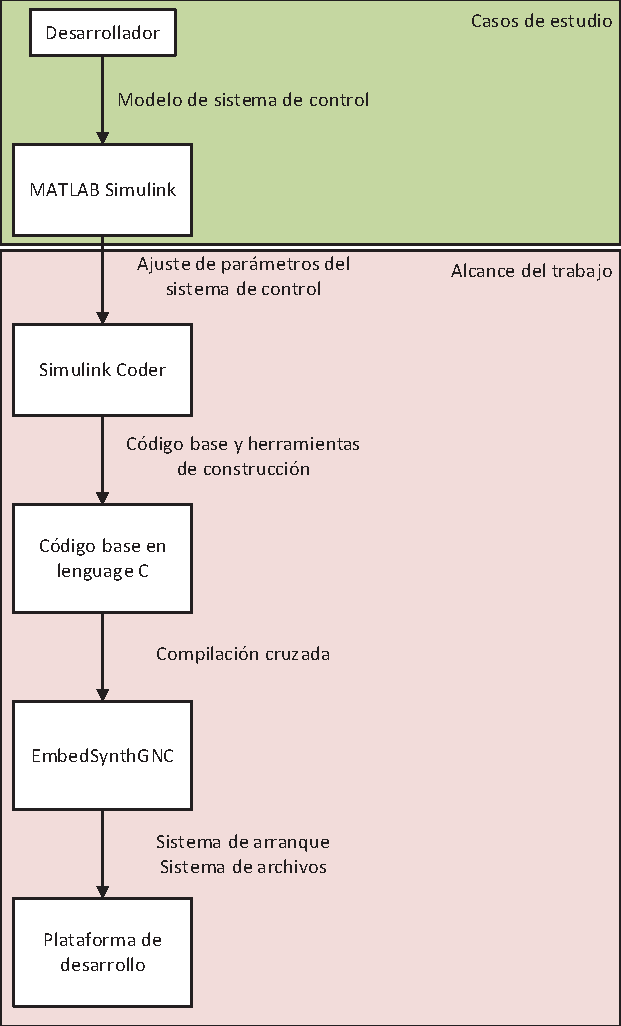
\includegraphics[scale=0.4]{Diagrama_general_del_proyecto/dgp_1.pdf}
\end{frame}

\begin{frame}{Diseño flujo de trabajo}
  \centering
  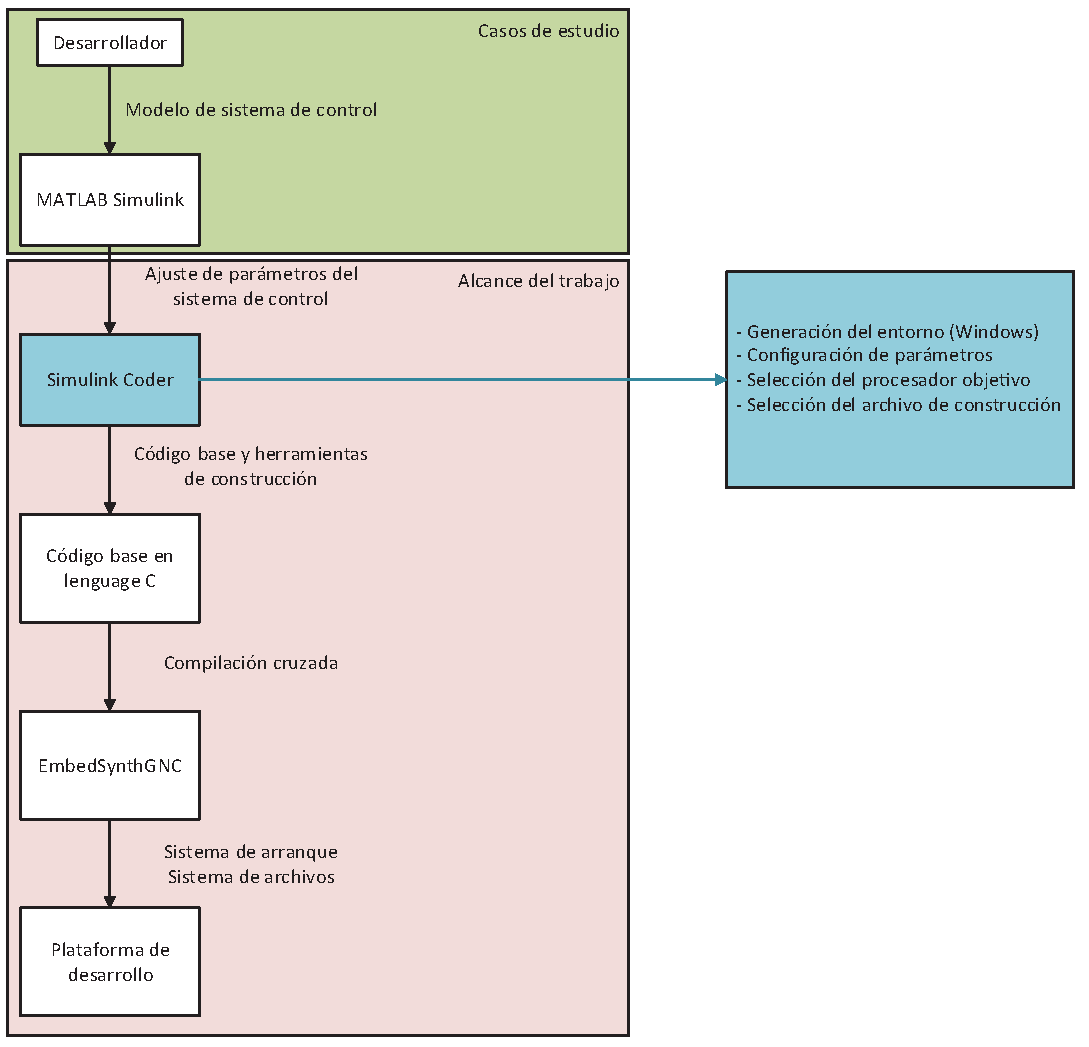
\includegraphics[scale=0.4]{Diagrama_general_del_proyecto/dgp_2.pdf}
\end{frame}

\begin{frame}{Diseño flujo de trabajo}
  \centering
  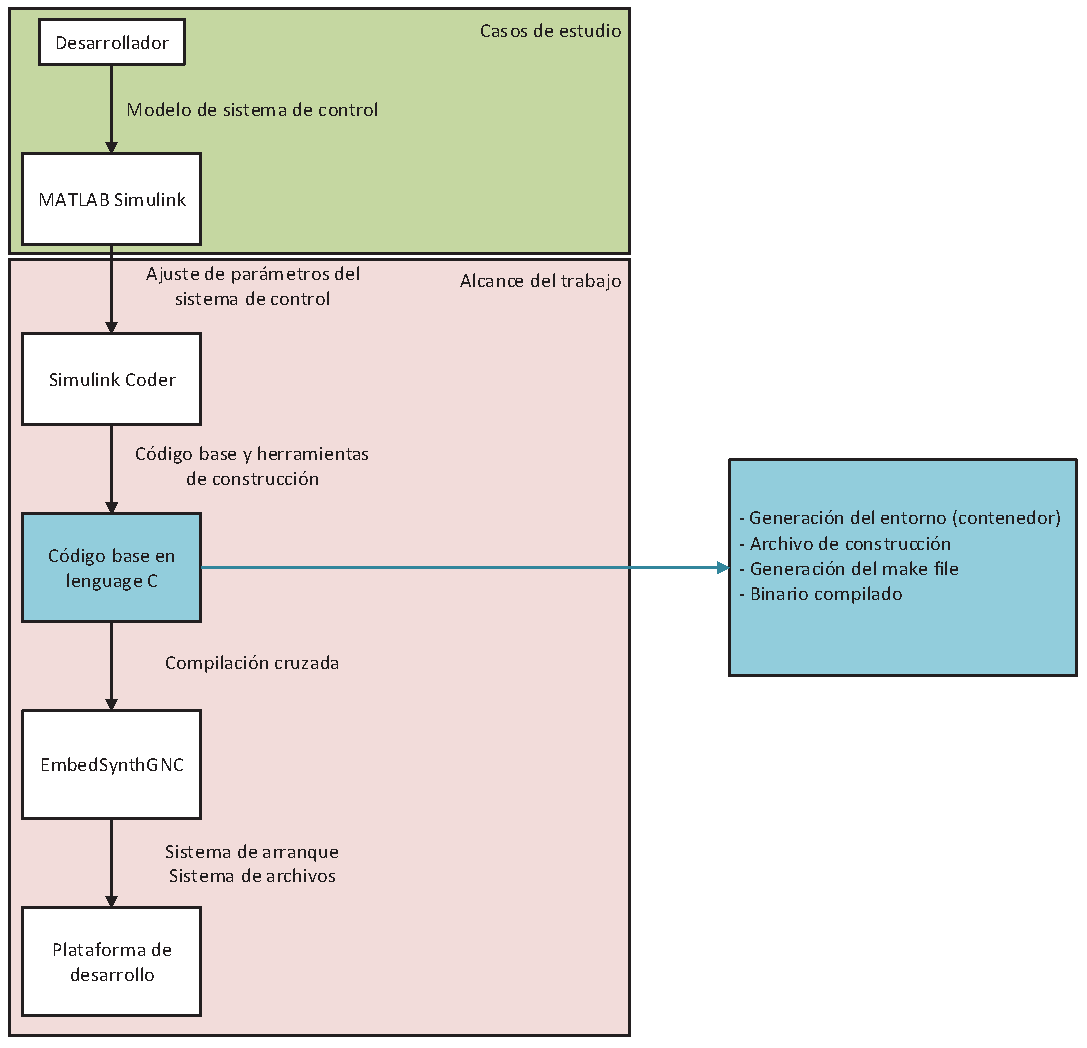
\includegraphics[scale=0.4]{Diagrama_general_del_proyecto/dgp_3.pdf}
\end{frame}

\begin{frame}{Diseño flujo de trabajo}
  \centering
  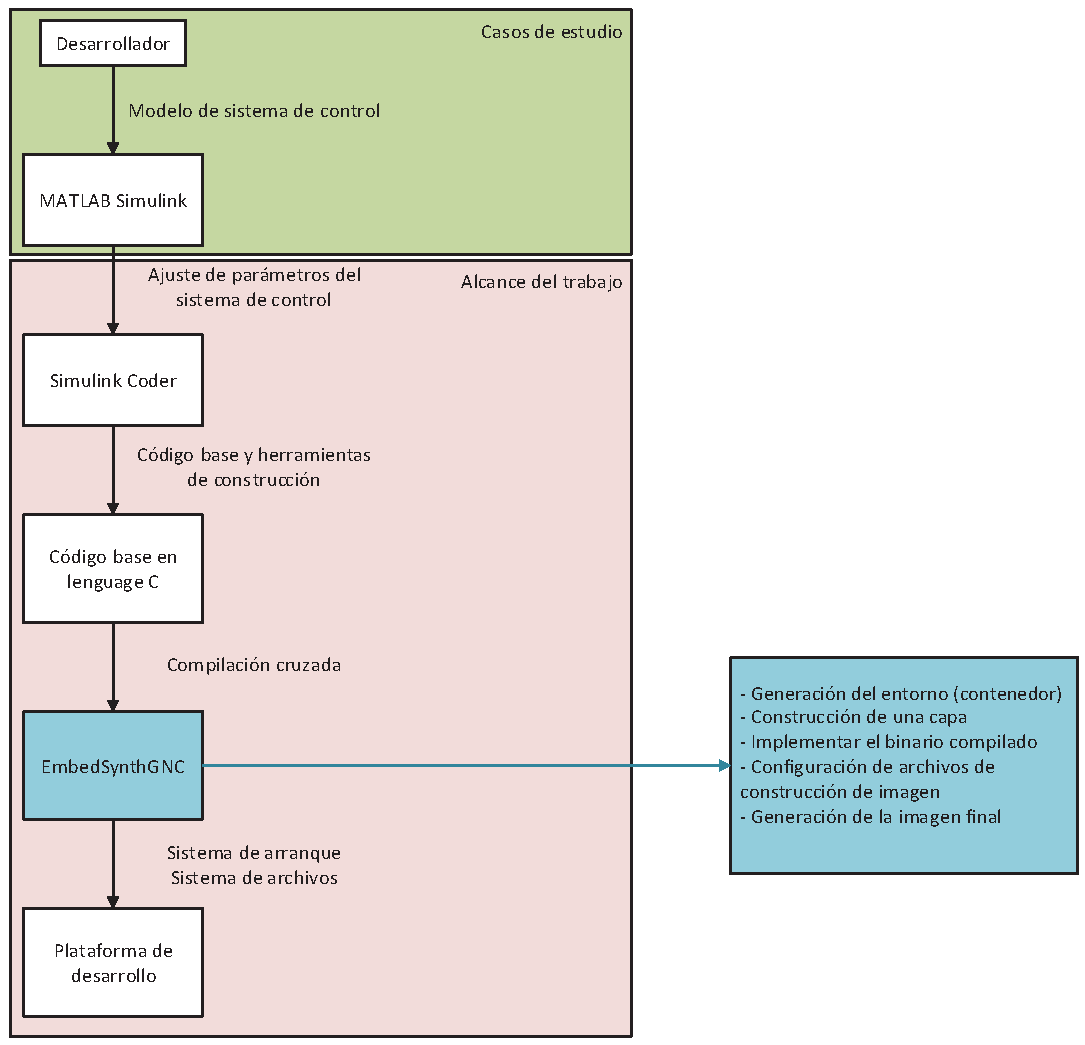
\includegraphics[scale=0.4]{Diagrama_general_del_proyecto/dgp_4.pdf}
\end{frame}

\begin{frame}{Diseño flujo de trabajo}
  \centering
  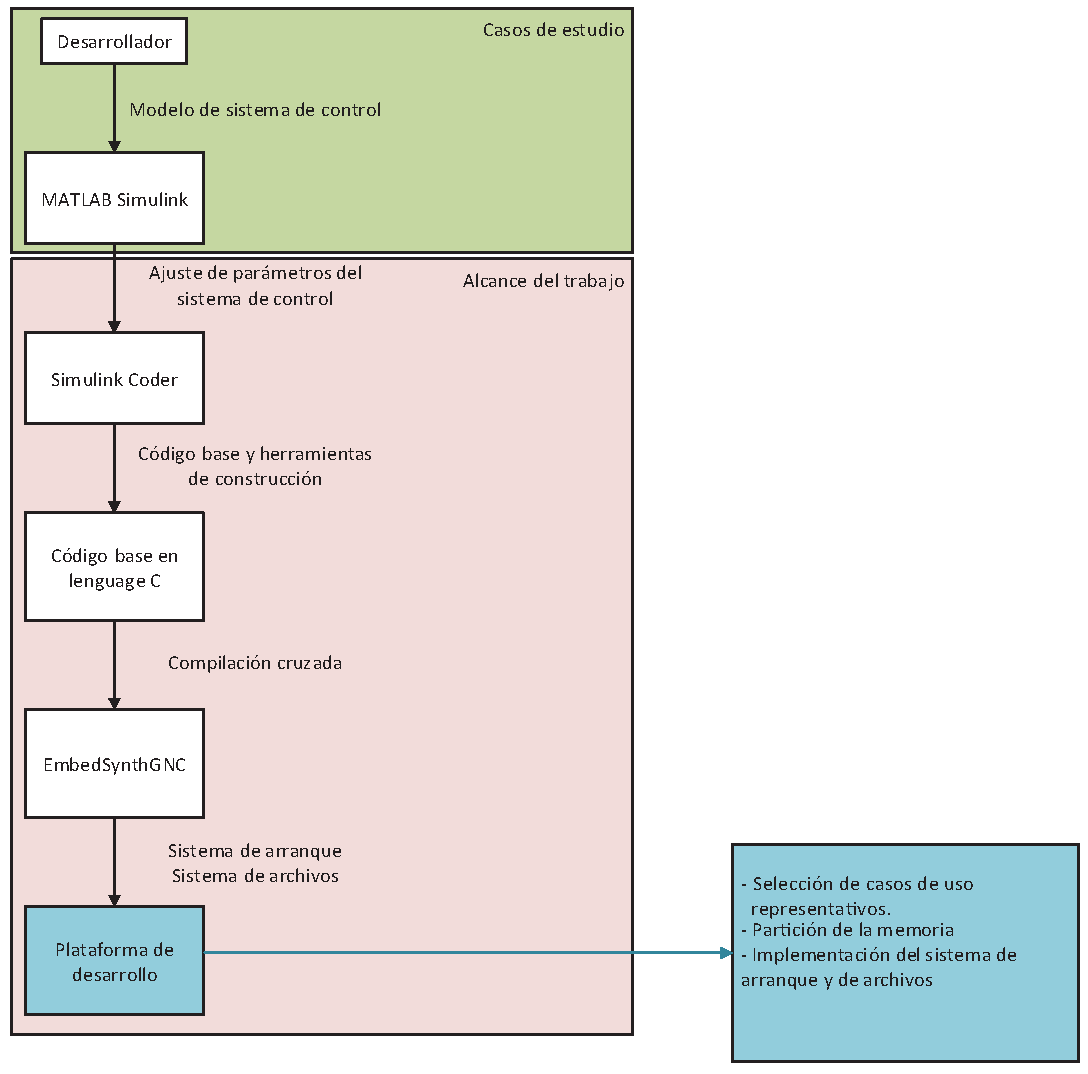
\includegraphics[scale=0.4]{Diagrama_general_del_proyecto/dgp5.pdf}
\end{frame}

\section{Casos de uso}

\subsection{Filtro}

\begin{frame}{Caso de uso - Filtro}
  \centering
  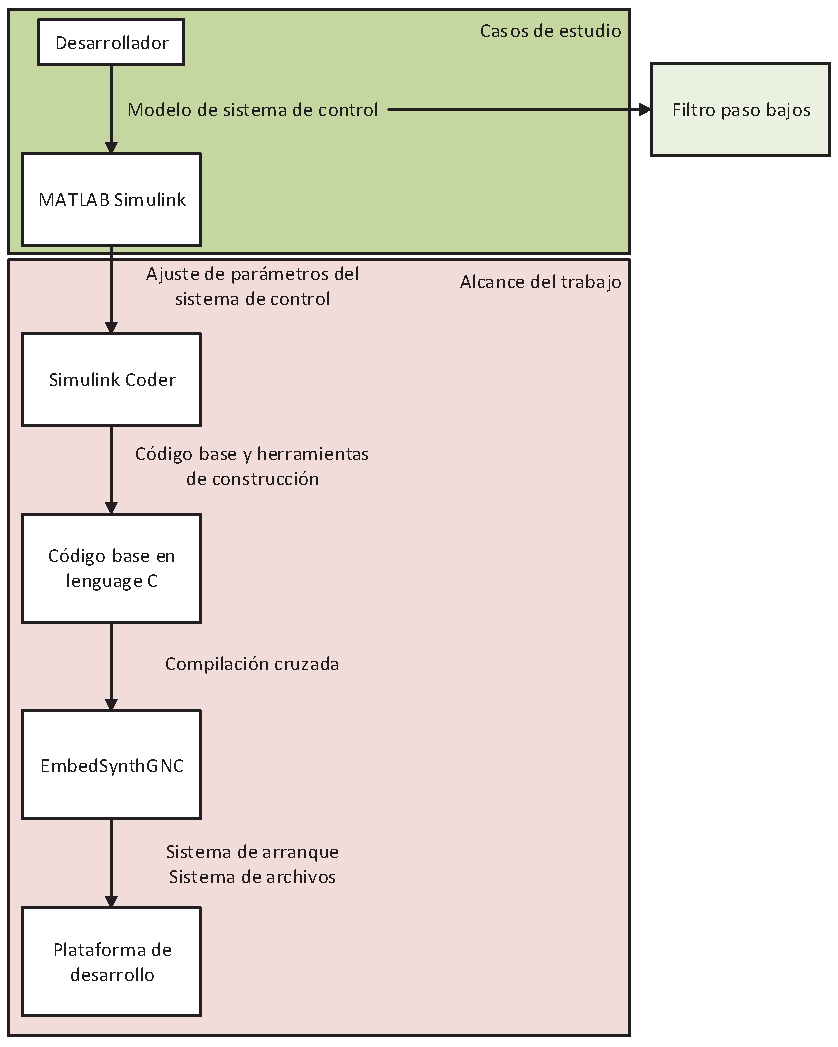
\includegraphics[scale=0.4]{Diagrama_general_del_proyecto/dgp_ce_2.pdf}
\end{frame}

\begin{frame}{Caso de uso - Filtro}
  \centering
  \begin{minipage}{0.45\linewidth}
    \centering
    \includegraphics[scale=0.15]{Filtro/raw_sim.png}
  \end{minipage}%
  \hfill
  \begin{minipage}{0.55\linewidth}
    \centering
    \includegraphics[scale=0.15]{Filtro/filt_sim.png}
  \end{minipage}
  \begin{minipage}{0.45\linewidth}
    \centering
    \includegraphics[scale=0.15]{Filtro/raw_exp.png}
  \end{minipage}%
  \hfill
  \begin{minipage}{0.55\linewidth}
    \centering
    \includegraphics[scale=0.15]{Filtro/filt_exp.png}
  \end{minipage}

  \vspace{0.5cm} % Espacio entre las imágenes y la tabla

    \begin{minipage}{0.9\linewidth} % Ajusta el ancho aquí
      \centering
      % Crea una tabla de 3x4 con contenido
      \begin{tabular}{ll}
        Métrica                       & Error \\ \hline
        Error promedio absoluto         &   $1.930 \times 10^{-18}$ [V]    \\
        Error cuadrático medio          &   $2.14 \times 10^{-34}$ $[V^{2}]$    \\
        Raíz del error cuadrático medio &   $1.46 \times 10{-17}$ [V]  
        \end{tabular}
    \end{minipage}
  
\end{frame}

\subsection{IMU}

\begin{frame}{Caso de uso - IMU}
  \centering
  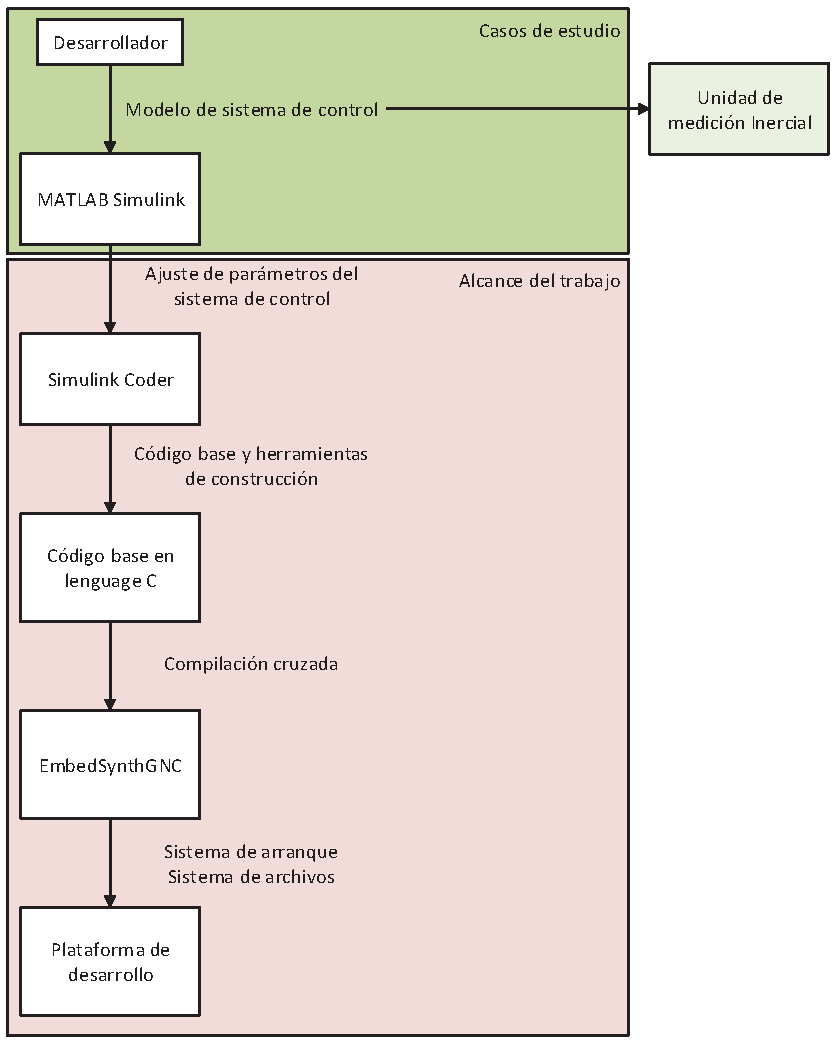
\includegraphics[scale=0.4]{Diagrama_general_del_proyecto/dgp_ce_3.pdf}
\end{frame}

\begin{frame}{Caso de uso - IMU}
  \centering
  \begin{minipage}{0.45\linewidth}
    \centering
    \includegraphics[scale=0.2]{IMU/simulated/error_de_orientacion_simulado.png}
  \end{minipage}%
  \hfill
  \begin{minipage}{0.45\linewidth}
    \centering
    \includegraphics[scale=0.2]{IMU/experimental/error_de_orientacion.png}
  \end{minipage}

  \vspace{0.5cm} % Espacio entre las imágenes y la tabla

  
    \begin{minipage}{0.9\linewidth} % Ajusta el ancho aquí
      \centering
      % Crea una tabla de 3x4 con contenido
      \begin{tabular}{ll}
        Métrica                       & Error \\ \hline
        Error promedio absoluto         &   $1.28 \times 10^{-13}$ [grados]\\
        Error cuadrático medio          &   $2.12 \times 10^{-13}$ $[grados^{2}]$    \\
        Raíz del error cuadrático medio &   $4.51 \times 10{-26}$ [grados]  
        \end{tabular}
    \end{minipage}
\end{frame}

\begin{frame}{Caso de uso - IMU}
  \centering
  \begin{minipage}{0.45\linewidth}
    \centering
    \includegraphics[scale=0.2]{IMU/simulated/sesgo_simulado.png}
  \end{minipage}%
  \hfill
  \begin{minipage}{0.45\linewidth}
    \centering
    \includegraphics[scale=0.2]{IMU/experimental/sesgo_experimental.png}
  \end{minipage}

  \vspace{0.5cm} % Espacio entre las imágenes y la tabla

  
    \begin{minipage}{0.9\linewidth} % Ajusta el ancho aquí
      \centering
      % Crea una tabla de 3x4 con contenido
      \begin{tabular}{ll}
        Métrica                       & Error \\ \hline
        Error promedio absoluto         &   $2.31 \times 10^{-15}$ [grados/s]    \\
        Error cuadrático medio          &   $3.09 \times 10^{-15}$ $[grados/s^{2}]$    \\
        Raíz del error cuadrático medio &   $9.56 \times 10{-30}$ [grados/s]  
        \end{tabular}
    \end{minipage}
\end{frame}


\subsection{PID}
\begin{frame}{Casos de uso - PID}
  \centering
  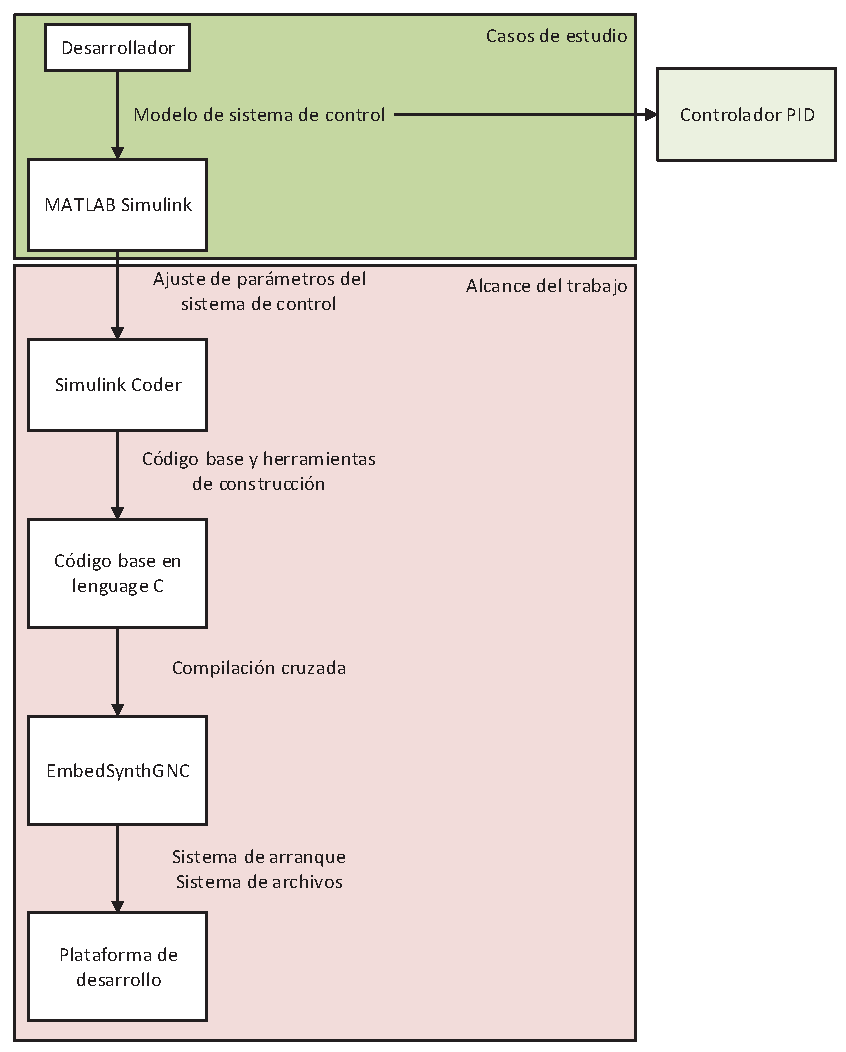
\includegraphics[scale=0.4]{Diagrama_general_del_proyecto/dgp_ce_1.pdf}
\end{frame}

\begin{frame}{Casos de uso - PID}
  \centering
  \begin{minipage}{0.4\linewidth}
    \centering
    \includegraphics[scale=0.2]{PID/entrada_simulada.png}
  \end{minipage}%
  \hfill
  \begin{minipage}{0.4\linewidth}
    \centering
    \includegraphics[scale=0.17]{PID/salida_simulada.png}
  \end{minipage}

  \vspace{0.1cm} % Espacio entre las imágenes y la tabla

  \begin{minipage}{0.4\linewidth}
    \centering
    \includegraphics[scale=0.2]{PID/entrada_experimental.png}
  \end{minipage}%
  \hfill
  \begin{minipage}{0.4\linewidth}
    \centering
    \includegraphics[scale=0.17]{PID/salida_experimental.png}
  \end{minipage}

  \vspace{0.2cm} % Espacio entre las imágenes y la tabla
    \begin{minipage}{0.9\linewidth} % Ajusta el ancho aquí
      \centering
      % Crea una tabla de 3x4 con contenido
      \begin{tabular}{ll}
        Métrica                       & Error \\ \hline
        Error promedio absoluto         &   $1.12\times 10^{-32}$ [V]\\
        Error cuadrático medio          &   $1.01 \times 10^{-34}$ $[V^{2}]$    \\
        Raíz del error cuadrático medio &   $1.01 \times 10{-17}$ [V]  
        \end{tabular}
    \end{minipage}
\end{frame}



\section{Conclusiones y recomentaciones}

\begin{frame}{Conclusiones}
  \begin{itemize}
    \item Se seleccionó la plataforma embebida ZedBoard debido a su desempeño y compatibilidad con plataformas espaciales como el computador a bordo ICEPS de EXA.
    \item Se desarrolló un entorno de compilación cruzada para convertir el código generado en un archivo binario para la arquitectura ARM.
    \item Se desarrolló un entorno de trabajo para la síntesis de archivos de arranque y archivos de sistema para la plataforma embebida ZedBoard.
    \item Se desarrollaron tres algoritmos básicos  de control como casos de uso para aplicaciones GNC uno orientado al filtrado de señales, otro orientado a estimación de estado y otro a control.
  \end{itemize}
\end{frame}

\begin{frame}{Recomendaciones y trabajo futuro}
  \begin{itemize}
    \item Realizar una evaluación comparativa continua del desempeño de la ZedBoard frente a nuevas plataformas de hardware embebido para mantener actualizado el sistema, considerando nuevas opciones con mayores capacidades o eficiencia energética, especialmente si surgen otros modelos compatibles con ICEPS de EXA.
    \item Automatizar el entorno de compilación cruzada mediante scripts y herramientas como CE Docker, para facilitar la generación de binarios para ARM y simplificar la integración de futuros cambios en el código.
  \end{itemize}
\end{frame}

\begin{frame}{Recomendaciones y trabajo futuro}
  \begin{itemize}
    \item Implementar un sistema de versionado y pruebas automatizadas para los archivos de arranque y de sistema. Esto permitirá asegurar la compatibilidad y estabilidad del entorno a lo largo del ciclo de vida del proyecto y en futuras iteraciones.
    \item Diseñar un marco de validación de algoritmos que permita evaluar la efectividad de cada algoritmo de control en simulaciones y pruebas de hardware en lazo cerrado. Esto ayudará a identificar mejoras en su rendimiento y adaptabilidad para aplicaciones GNC complejas.
  \end{itemize}
\end{frame}


\end{document}
